\FloatBarrier
\section{Matched absolute-pin witness comparison}
\label{app:pin-quality-v3}
The completed \texttt{chess-pin-quality-v3} study tests whether joint processing
of rule-derived king, blocker and attacker witnesses improves candidate ranking
beyond the established graph-difference path and simpler controls. It is
\emph{adaptive development on previously exposed panels}, not independent
confirmation. All eight arms use the same authenticated canonical root features,
legal menus, complete native child graphs and pin-factor inputs, with the
information restrictions appropriate to each control. The designated treatment
is the joint pin-factor head. Comparators are WLDN, first-order separable and
pairwise factor heads, root-only pin context, six owner/status pin counts, a
graph MLP without witnesses, and the previously selected edit-labelled union
head. The frozen backbone is evaluated separately for every seed.

\paragraph{Matched recipe, unequal computation.}
All 24 fits use seeds 97, 109 and 127, with 32,768 training roots, six epochs,
batch size 128, and 1,536 Adam updates each. Every fit starts fresh and all
training finishes before evaluation. The recipe fixes the learning rate at
$10^{-3}$, gradient clipping at one and legal-menu cross entropy; it does not
select checkpoints by evaluation results. The stored head sizes range from
16,638 to 16,740 parameters. This proximity does not equalize active capacity,
FLOPs or optimization. In particular, the pairwise restriction applies inside
the anchored factor MLP, not to all policy interactions. Pooling a named motif
does not itself establish a new architecture family.

% Generated by write_pin_quality_v3.py from hash-bound saved evidence.
\begin{table}[ht]
\centering\small
\caption{Matched pin-quality v3. Means over all three seeds; agreement is
in percent and target NLL in nats. Each exposed development panel has
2,048 roots. All eight trained arms and all three frozen backbones are
retained; the designated joint arm fails its quality criterion.}
\label{tab:pin-quality-v3}
\begin{tabular}{lrrrr}
\toprule
& \multicolumn{2}{c}{Agreement (\%)} & \multicolumn{2}{c}{Target NLL} \\
Method & Ordinary & Shift & Ordinary & Shift \\
\midrule
Frozen backbone & 31.755 & 26.807 & 2.434607 & 2.634750 \\
WLDN & 37.158 & 31.917 & 2.153503 & 2.348466 \\
Joint pin & 36.426 & 31.396 & 2.172513 & 2.368147 \\
Separable & 37.012 & 31.510 & 2.161526 & 2.358588 \\
Pairwise & 36.572 & 31.445 & 2.165616 & 2.348599 \\
Root only & 36.751 & 31.462 & 2.169414 & 2.366796 \\
Counts & 36.637 & 31.608 & 2.152418 & 2.352115 \\
Graph MLP & 36.572 & 31.657 & 2.166158 & 2.366070 \\
Union edits & 36.686 & 31.657 & 2.165127 & 2.360217 \\
\bottomrule
\end{tabular}
\end{table}


\paragraph{The original criterion fails.}
Only \PinQualityChecksPassed{}/\PinQualityChecksTotal{} checks pass, both against
the frozen backbone. The joint arm has lower mean agreement than every trained
comparator on both panels (Table~\ref{tab:pin-quality-v3-checks}). Its gains over
the frozen backbone therefore do not establish a benefit of the proposed
joint mechanism. The continuation criterion remains failed; WLDN cannot be
substituted as the designated treatment after observing these results.

% Generated by write_pin_quality_v3.py from hash-bound saved evidence.
\begin{table}[ht]
\centering\small
\caption{All sixteen original joint-minus-comparator quality checks.
Mean gain and worst paired-seed gain are percentage points. Every
check requires a paired-seed floor of $-0.5$ points; mean gain must
be at least zero against the backbone and $+1.0$ against trained controls.}
\label{tab:pin-quality-v3-checks}
\begin{tabular}{llrrc}
\toprule
Panel & Comparator & Mean gain & Worst seed & Check \\
\midrule
Ordinary & Frozen backbone & +4.671 & +4.102 & Pass \\
Ordinary & WLDN & -0.732 & -1.562 & Fail \\
Ordinary & Separable & -0.586 & -1.123 & Fail \\
Ordinary & Pairwise & -0.146 & -0.391 & Fail \\
Ordinary & Root only & -0.326 & -0.537 & Fail \\
Ordinary & Counts & -0.212 & -0.879 & Fail \\
Ordinary & Graph MLP & -0.146 & -0.586 & Fail \\
Ordinary & Union edits & -0.260 & -0.635 & Fail \\
Shift & Frozen backbone & +4.590 & +3.662 & Pass \\
Shift & WLDN & -0.521 & -2.100 & Fail \\
Shift & Separable & -0.114 & -0.391 & Fail \\
Shift & Pairwise & -0.049 & -0.928 & Fail \\
Shift & Root only & -0.065 & -0.439 & Fail \\
Shift & Counts & -0.212 & -0.732 & Fail \\
Shift & Graph MLP & -0.260 & -0.928 & Fail \\
Shift & Union edits & -0.260 & -1.270 & Fail \\
\bottomrule
\end{tabular}
\end{table}

\FloatBarrier

\begin{figure}[ht]
\centering
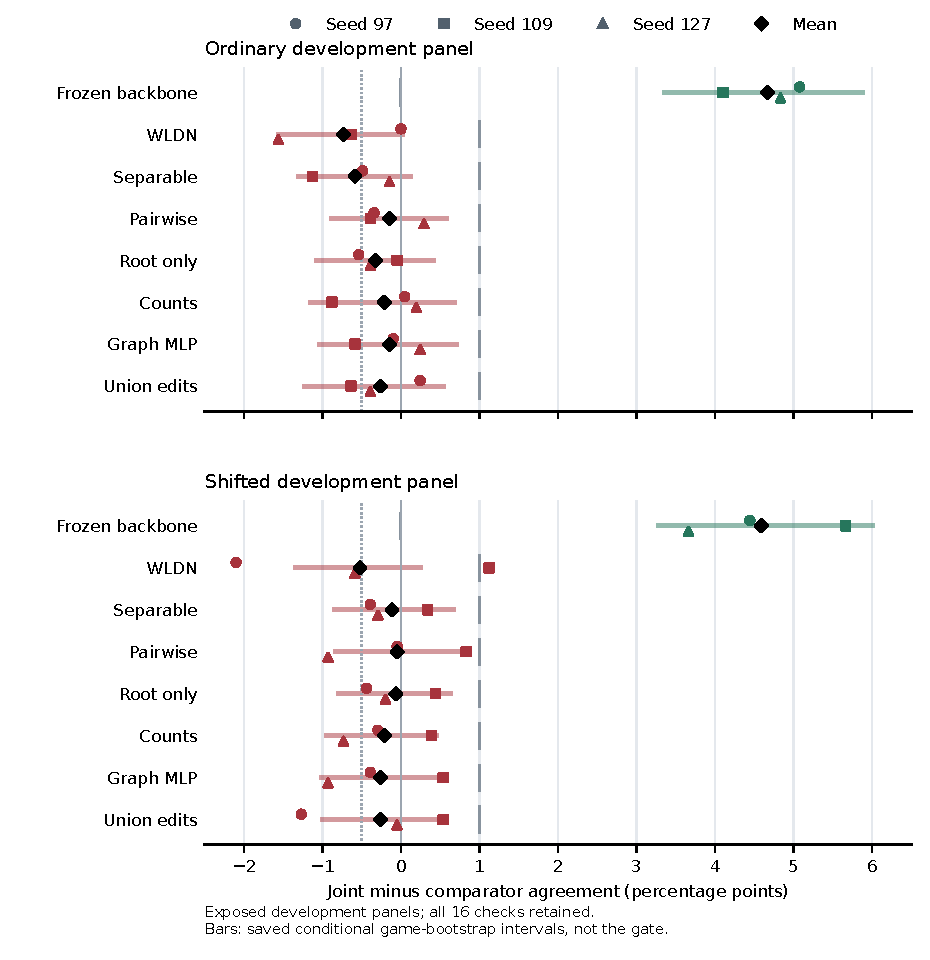
\includegraphics[width=\linewidth]{pin-quality-v3-comparisons.pdf}
\caption{All paired seed differences for the original sixteen comparisons.
The figure uses the authenticated completed audit report without new scoring
or resampling. Symbols retain all three seeds; bars are conditional source-game
bootstrap intervals. Green/red denotes the full check passing/failing. Short
vertical ticks mark required means and the dotted line the paired-seed floor.
These are previously exposed development data.}
\label{fig:pin-quality-v3-checks}
\end{figure}

\paragraph{Conditional uncertainty.}
The saved audit also recomputes all sixteen 95\% source-game bootstrap
intervals, using 2,000 draws and averaging the three paired-seed correctness
differences within each root before position-weighting sampled games. There
are 39 source games in the ordinary panel and 31 in the shifted panel, each
with 2,048 roots. These intervals describe the fixed trained models and exposed
panels. They include neither uncertainty over new training seeds nor correction
for adaptive development or multiple comparisons. They are not a substitute for
the failed original continuation rule.

\paragraph{Audit scope and numerical agreement.}
The completed audit authenticates source, input and execution manifests, all
24 initial and final checkpoint identities, and 36,864 training-index receipts.
It replays 110,592 prediction records and 3,226,149 legal-candidate scores,
including 12,288 native root/backbone reconstructions. It recomputes all cached
scores and target NLLs exactly, and reproduces native vectors and comparisons
with the same production neural kernels. The native/cached numerical gate
passes: the maximum score discrepancy is $3.8146973\times10^{-6}$, below
$10^{-5}$, with zero failed method-position cases and zero changed choices.
This audit is not an independent neural implementation or a repeat of training.
The table and figure generators perform no new model or engine calls.

\paragraph{Elapsed costs and incomplete earlier attempts.}
Execution took \PinQualityExecutionSeconds{} seconds and the separate audit
\PinQualityAuditSeconds{} seconds. The \PinQualityFitSeconds{} seconds summed
over fit receipts are nested inside execution, not an additional cost. The
earlier pin-quality-v2 attempt stopped before evaluation after 8,239 logged
updates and five completed fits; its termination cause is unknown. Its
\PinQualityPriorLoggedSeconds{} logged update seconds are a lower bound, and
the overlapping \PinQualityPriorFitSeconds{} completed-fit seconds must not be
added to that bound. Pin-quality-v1 stopped after 770 logged updates because a
game-ID validator rejected integer IDs, with no completed fit or quality
predictions. V3 restarts every fit; it reuses no earlier partial checkpoint.
These inputs do not quantify all historical project costs. Shared-host elapsed
times are not isolated inference latency or throughput measurements.

\paragraph{Separate complete native timing.}
The completed trained-head timing study evaluates all nine methods on 128
reused ordinary-panel roots, nine repeats and three seeds,
using the final V3 heads. Its 31,104 timings include complete native input
construction and scoring, with weights loaded outside the timed region.
Joint pin processing takes a median \PinCostJointMilliseconds{}\,ms, versus
\PinCostWLDNMilliseconds{}\,ms for WLDN. The median \emph{paired} joint/WLDN
ratio is \PinCostJointRatio{} (\PinCostJointPercent{}\% slower), rather than
the quotient of those marginal medians. All 54 warmups, timed outputs and
3,456 separately replayed audit decisions have zero score error and no changed
choices. These are descriptive shared-host measurements, not a cross-machine
speed comparison or throughput estimate. The added cost does not rescue the
failed quality criterion.

\paragraph{Reproduction and claim boundary.}
The saved quality protocol, numeric report and audit are retained under
\href{https://github.com/kw2828/OpenJev/tree/main/evidence/chess-pin-quality-v3}
{\texttt{chess-pin-quality-v3}} in the project evidence directory; the timing
study is under
\href{https://github.com/kw2828/OpenJev/tree/main/evidence/chess-pin-trained-cost-v2}
{\texttt{chess-pin-trained-cost-v2}}.
Their audit receipts begin \texttt{c86562f02e45} and \texttt{80415131be41}.
The separate manuscript table receipt binds full audit, figure and source
hashes. The publication helper \path{write_pin_quality_v3.py} checks those
identities before producing
Tables~\ref{tab:pin-quality-v3} and~\ref{tab:pin-quality-v3-checks}.
These results establish neither Elo nor gameplay strength, a general speed
advantage, independent confirmation, biological superiority or a novel mechanism
advantage.
\FloatBarrier
